\documentclass[en,hazy,device=normal,blue,14pt]{elegantnote}
%device for Pad(default), Kindle, PC, A4, 4:3 screen as pad, kindlle, pc, normal, screen
%math for defalut, newtxmath, mtpro2 as cm, newtx, mtpro2
%chinesefont for as ctexfont, founder, nofont
%color for blue(default), green, cyan, sakura and black
%lang for English and Chinese as en and cn

%定理类:theorem,lemma,proposition,corollary;
%定义类:definition,conjecture,example;
%备注类:remark,note,case;
%证明类:proof。
%lstlisting环境可用(lstinline行间代码)

\usepackage{ulem}%下划线uline

%\title{Chap9}

%\author{Chen Ziming}
%\institute{Elegant\LaTeX{} Program}

%\version{2.30}
%\date{\today}

\begin{document}
%\maketitle
% logo
%\centerline{
\includegraphics[width=0.2\textwidth]{logo-blue}}
\section{Chap9}
\subsection{THE WAVEFRONT RECONSTRUCTION PROBLEM}
\subsubsection{Recording Amplitude and Phase}
%\thispagestyle{empty}
Recording media respond to light intensity, using \textbf{interferometry} technique to record phase information.

Two complex fields are:
\begin{equation}
  \text{Unknown field:}\quad a\left( {x,y} \right) = \left| {a\left( {x,y} \right)} \right|\exp \left[ { - i\phi \left( {x,y} \right)} \right],
\end{equation}
\begin{equation}
  \text{Reference field:}\quad A\left( {x,y} \right) = \left| {A\left( {x,y} \right)} \right|\exp \left[ { - i\psi \left( {x,y} \right)} \right].
\end{equation}

The intensity of sum is 
\begin{equation}
  I\left( {x,y} \right) = {\left| {A\left( {x,y} \right)} \right|^2} + {\left| {a\left( {x,y} \right)} \right|^2} + 2\left| {A\left( {x,y} \right)} \right|\left| {a\left( {x,y} \right)} \right|\cos \left[ {\psi \left( {x,y} \right) - \phi \left( {x,y} \right)} \right].
\end{equation}
\begin{figure}[htbp]
  \centering
  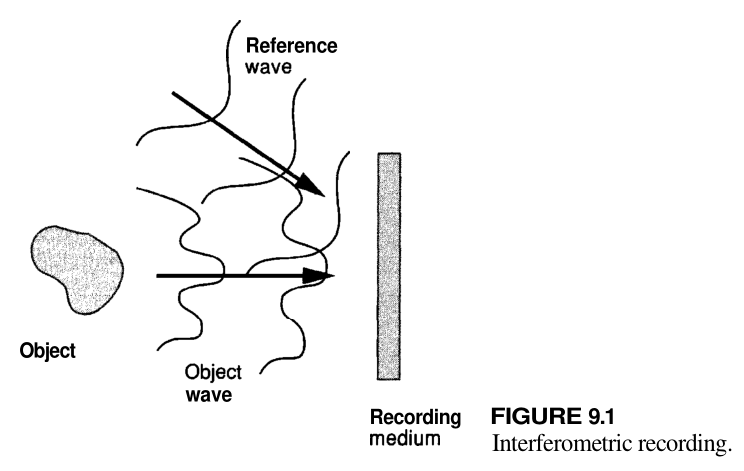
\includegraphics[width=0.7\textwidth]{1.png}
\end{figure}
\subsubsection{The Recording Medium}
Assume that the variations of exposure in the interference pattern remain within a linear region of the $t_A$ vs. $E$ curve.
\begin{equation}
  t_A\left(x,y\right)=t_b+\beta'\left(\left|a\right|^2+A^*a+Aa^*\right).
\end{equation}
Here $t_b$ is the uniform bias transmittance established by the constant reference exposure, and $\beta'$ is the product of the slope $\beta$ of the $t_A$ vs. $E$ curve at the bias point and the exposure time.
\subsubsection{Reconstruction of the Original Wavefront}
Suppose that the developed transparency is illuminated by a coherent reconstruction wave $B(x, y)$. The light transmitted by the transparency is evidently
\begin{equation}
  \begin{array}{c}
    B\left( {x,y} \right){t_A}\left( {x,y} \right) = {t_b}B + \beta 'a{a^*}B + \beta '{A^*}Ba + \beta 'AB{a^*}\\
     = {U_1} + {U_2} + {U_3} + {U_4}.
    \end{array}.
\end{equation}
\begin{itemize}
  \item If $B$ is the exact duplication of the original uniform reference wavefront $A$, the third term of this equation becomes
  \begin{equation}
    U_3\left(x,y\right)=\beta'\left|A\right|^2a\left(x,y\right),
  \end{equation}
  \item If $B$ is the conjugate of the original reference wave, i.e. as $A^*(x, y)$, the fourth term of the reconstructed field becomes
  \begin{equation}
    {U_4}\left( {x,y} \right) = \beta '{\left| A \right|^2}{a^*}\left( {x,y} \right).
  \end{equation}
\end{itemize}

\begin{figure*}[htbp]
  \centering
  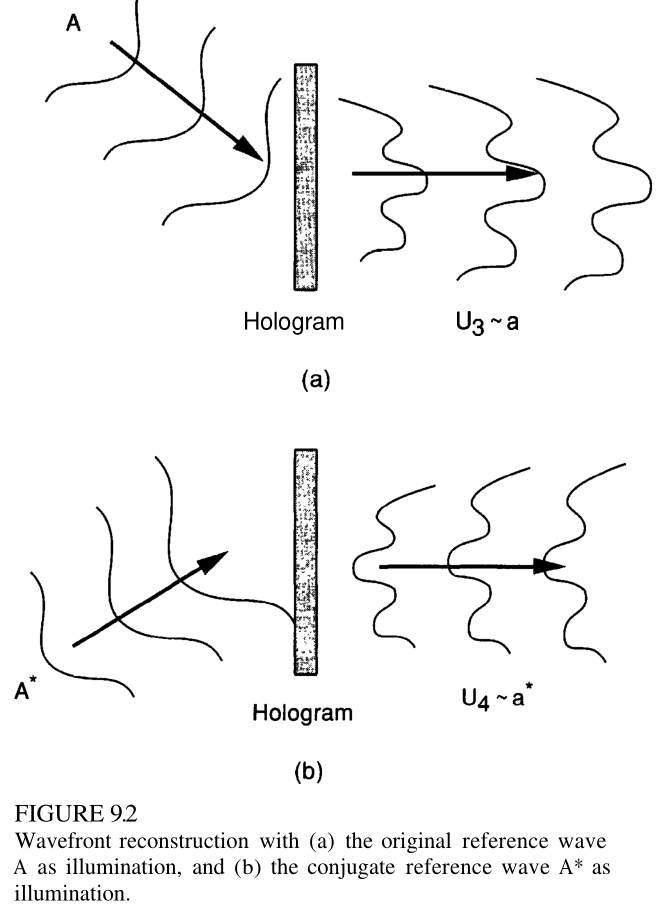
\includegraphics[width=0.7\textwidth]{2.png}
\end{figure*}

\subsubsection{Linearity of the Holographic Process}
\uline{The linear system concept plays no role in holography.}

The nonlinearity of the detection process manifests itself in the generation of several output terms, but there is no nonlinear distortion of the one term of interest, assuming that the exposure variations remain in the linear region of the $t_A$ vs. $E$ curve.

\subsubsection{Image Formation by Holography}
Considered only the problem of reconstructing a wavefront which arrived at a recording medium from a coherently illuminated object
\begin{itemize}
  \item In Figure3(b), we see that the wave $U_3$ under reconstruction field $A$ can be seen as a \textbf{duplication} of the object and as a \textbf{virtual object};
  \item In Figure 3(c), we see that the wave $U_4$ under reconstruction field $A^*$ can generate a \textbf{real image}.
\end{itemize}

\begin{example}
  If we consider that the object field is 
  \begin{equation}
    a\left( {x,y} \right) = {a_0}\exp \left[ {ik\sqrt {z_0^2 + {{\left( {x - {x_0}} \right)}^2} + {{\left( {y - {y_0}} \right)}^2}} } \right],
  \end{equation}
  then we can see that under two reconstruction field $U_3$ and $U_4$ will be
  \begin{equation}
    U_3\left(x,y\right)=\beta'\left|A\right|^2{a_0}\exp \left[ {ik\sqrt {z_0^2 + {{\left( {x - {x_0}} \right)}^2} + {{\left( {y - {y_0}} \right)}^2}} } \right],
  \end{equation}
  and
  \begin{equation}
    {U_4}\left( {x,y} \right) = \beta '{\left| A \right|^2}{a_0}\exp \left[ {-ik\sqrt {z_0^2 + {{\left( {x - {x_0}} \right)}^2} + {{\left( {y - {y_0}} \right)}^2}} } \right].
  \end{equation}
\end{example}
\begin{figure}[htbp]
  \centering
  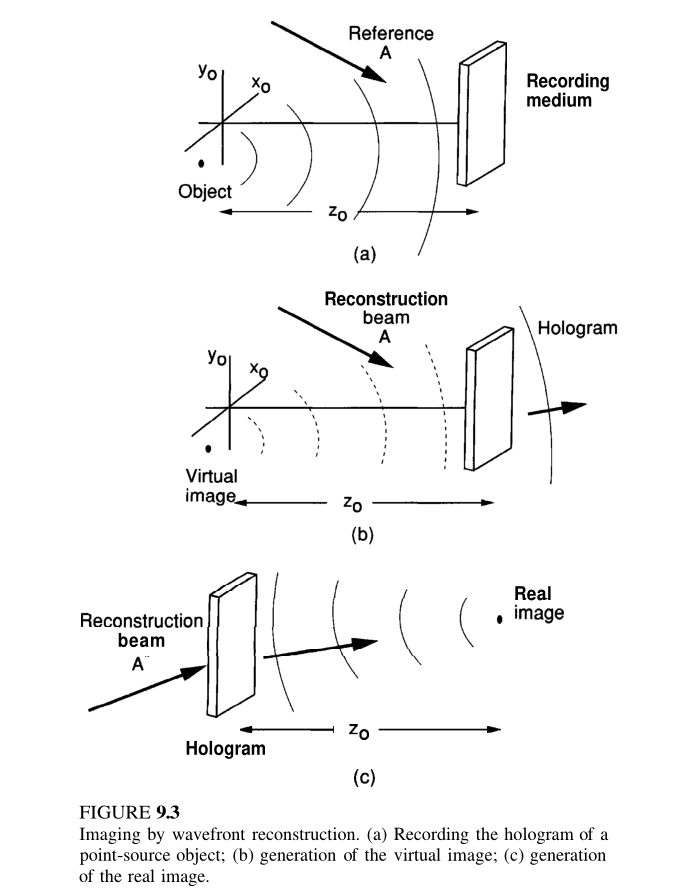
\includegraphics[width=0.7\textwidth]{3.png}
\end{figure}

\subsection{THE GABOR HOLOGRAM}
\subsubsection{Origin of the Reference Wave}
Object assumed to be highly transmissive, with an amplitude transmittance
\begin{equation}
  t\left( {{x_o},{y_o}} \right) = {t_0} + \Delta t\left( {{x_o},{y_o}} \right),
\end{equation}
where the variation is smaller than the average.

When such an object is coherently illuminated by the collimated wave shown in Fig.9.4, the transmitted light consists of two components: \uline{(1) a strong uniform plane wave passed by the term $t_0$, and (2) a weak scattered wave generated by the transmittance variations $\Delta t\left( {{x_o},{y_o}} \right)$.}

Then the medium records the intensity as
\begin{equation}
  I\left( {x,y} \right) = {\left| {A} \right|^2} + {\left| {a\left( {x,y} \right)} \right|^2} + A^*a\left(x,y\right)+Aa^*\left(x,y\right),
\end{equation}
Here $A$ is the amplitude of the plane wave and $a$ is the scattered field.

\begin{figure}[htbp]
  \centering
  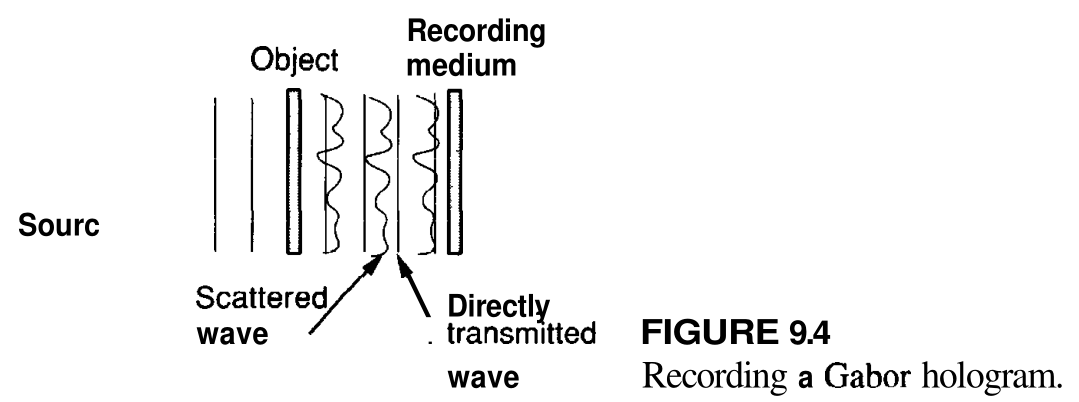
\includegraphics[width=0.7\textwidth]{4.png}
\end{figure}

\subsubsection{The Twin Images}
Using the plane wave $B$ to illuminate the medium, then the field will be
\begin{equation}
  B\left( {x,y} \right){t_A}\left( {x,y} \right) = B{t_b} +  \beta'B{\left| {a\left( {x,y} \right)} \right|^2} + \beta'A^*Ba\left(x,y\right)+\beta'ABa^*\left(x,y\right).
\end{equation}
\begin{itemize}
  \item The first term is a plane wave which passes directly through the transparency, suffering uniform attenuation but without scattering.
  \item The second term may be dropped as negligible by virtue of our assumption $\left|\Delta t\right|<\left|t_0\right|$, which implies that
  \begin{equation}
    \left| {a\left( {x,y} \right)} \right| \ll A.
  \end{equation}
  \item The third term represents a field component that is proportional to the original scattered wave $a(x, y)$. This wave appears to originate from a \textbf{virtual image} of the original object located at distance $z_o$ from the transparency.
  \item The fourth term is proportional to $a^*(x, y)$ and, in accord with our earlier discussions, leads to the formation of a \textbf{real image} at distance $z_o$ on the opposite side of the transparency from the virtual image.
\end{itemize}

\begin{figure}[htbp]
  \centering
  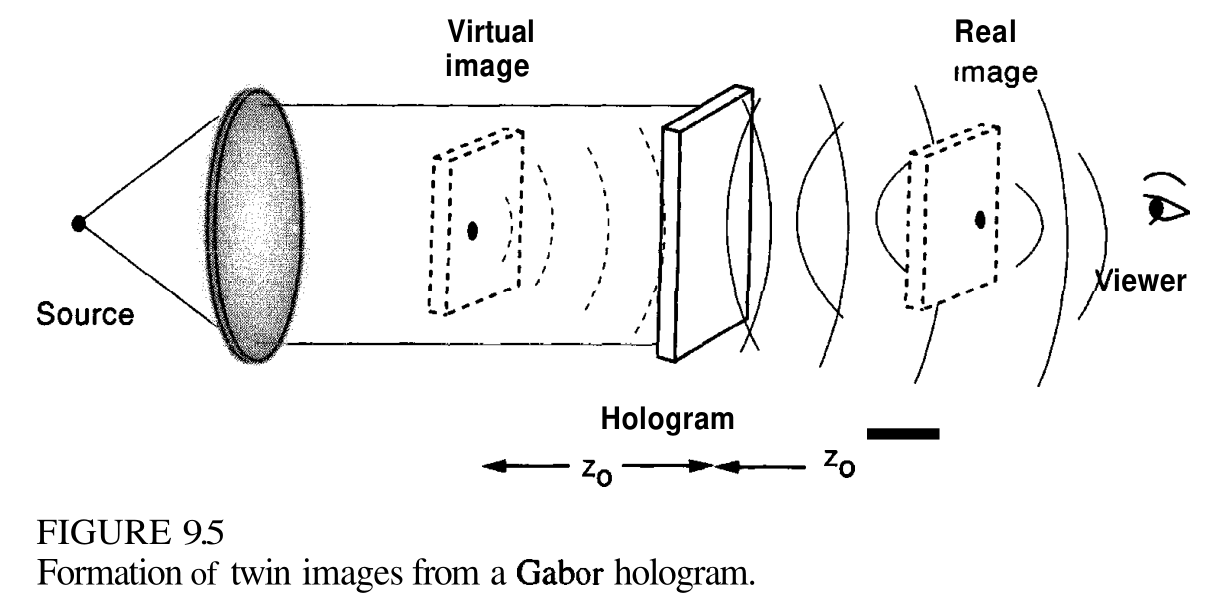
\includegraphics[width=0.7\textwidth]{5.png}
\end{figure}

\subsubsection{Limitations of the Gabor Hologram}
\begin{itemize}
  \item The most important limitation is inherent in the assumption of a highly transparent object and the consequent conclusion $\left| {a\left( {x,y} \right)} \right| \ll A$ that followed.
  $\to$ Then the second term will remain 
  \begin{equation}
    U_2=\beta'B{\left| {a\left( {x,y} \right)} \right|^2}.
  \end{equation}
  \uline{Low average transmittance lead to $U_2$ to be the largest contributing term.} So Gabor Hologram can be applied with opaque letters on a transparent background, but not with not transparent letters on an opaque background. 
  \item A second serious limitation lies in the generation of \textbf{overlapping twin images}, rather than a single image. When the real image is brought to focus, it is always accompanied by an out-of-focus virtual image. Likewise an observer viewing the virtual image sees simultaneously a defocused image arising from the real-image term. Thus, even for highly transparent objects, the quality of the images is reduced by the twin image problem.
\end{itemize}

\subsection{THE LEITH-UPATNIEKS HOLOGRAM}
The major change between this type of hologram and the Gabor hologram is that, rather than depending on the light directly transmitted by the object to serve as a reference wave, a \textbf{separate and distinct reference} wave is introduced.
Furthermore the reference is introduced at an
offset angle, rather than being collinear with the object-film axis.

\subsubsection{Recording the Hologram}
\begin{figure}[htbp]
  \centering
  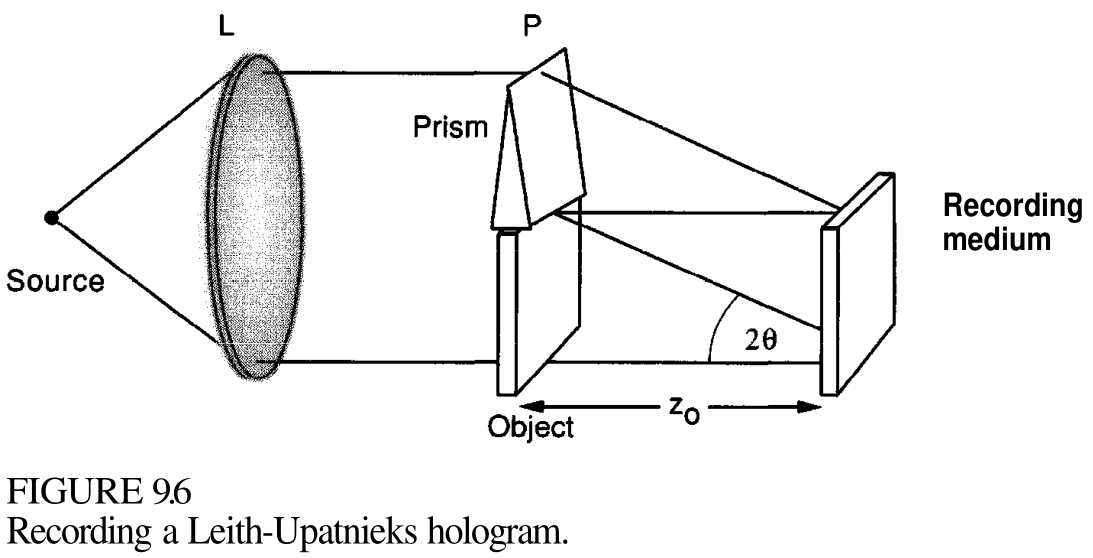
\includegraphics[width=0.7\textwidth]{6.PNG}
\end{figure}

On the recording plane
\begin{equation}
  U\left( {x,y} \right) = A\exp \left( { - j2\pi \alpha y} \right) + a\left( {x,y} \right),
\end{equation}
where 
\begin{equation}
  \alpha = \frac {\sin2\theta}{\lambda}.
\end{equation}

Then the intensity distribution across the recording plane is evidently
\begin{equation}
  I\left( {x,y} \right) = {\left| A \right|^2} + {\left| {a\left( {x,y} \right)} \right|^2} + {A^*}a\left( {x,y} \right)\exp \left( {j2\pi \alpha y} \right) + A{a^*}\left( {x,y} \right)\exp \left( { - j2\pi \alpha y} \right).
\end{equation}
If the object field is expressed by the modula and the phase
\begin{equation}
  a\left( {x,y} \right) = \left| {a\left( {x,y} \right)} \right|\exp \left[ { - j\phi \left( {x,y} \right)} \right],
\end{equation}
then the intensity will be
\begin{equation}
  I\left( {x,y} \right) = {\left| A \right|^2} + {\left| {a\left( {x,y} \right)} \right|^2} + 2\left| A \right|\left| {a\left( {x,y} \right)} \right|\cos \left[ {2\pi \alpha y - \phi \left( {x,y} \right)} \right].
\end{equation}
This expression demonstrates that the amplitude and phase of the light arriving from the object have been recorded, respectively, \uline{as amplitude and phase modulations of a spatial carrier of frequency $\alpha$.} If the carrier frequency is sufficiently high, \uline{the amplitude and phase distributions can be unambiguously
recovered from this pattern of interference.}

\subsubsection{Obtaining the Reconstructed Images}
Like before, we find that the transmittance is
\begin{equation}
  {t_A}\left( {x,y} \right) = {t_b} + \beta '\left[ {{{\left| {a\left( {x,y} \right)} \right|}^2} + {A^*}a\left( {x,y} \right)\exp \left( {j2\pi \alpha y} \right) + A{a^*}\left( {x,y} \right)\exp \left( { - j2\pi \alpha y} \right)} \right].
\end{equation}
The four terms can be represented as
\begin{equation}
  \begin{array}{*{20}{c}}
    {{t_1} = {t_b},}&{{t_2} = \beta '{{\left| {a\left( {x,y} \right)} \right|}^2},}\\
    {{t_3} = \beta '{A^*}a\left( {x,y} \right)\exp \left( {j2\pi \alpha y} \right),}&{{t_4} = \beta' A{a^*}\left( {x,y} \right)\exp \left( { - j2\pi \alpha y} \right).}
    \end{array}
\end{equation}

\begin{figure}[htbp]
  \centering
  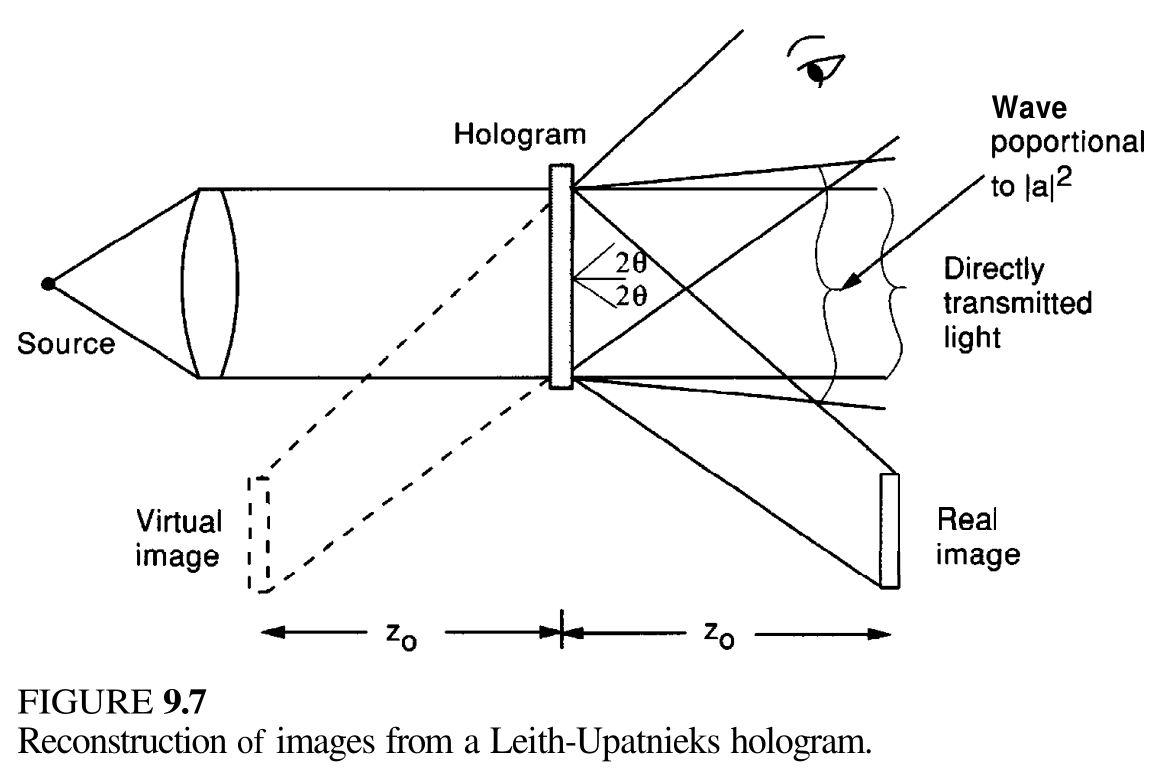
\includegraphics[width=0.7\textwidth]{7.png}
\end{figure}

Considering a normal incident light plane wave $B$, the transimitted wave will be
\begin{equation}
  \begin{array}{*{20}{c}}
    {{U_1} = {t_b}B,}&{{U_2} = \beta 'B{{\left| {a\left( {x,y} \right)} \right|}^2},}\\
    {{U_3} = \beta 'B{A^*}a\left( {x,y} \right)\exp \left( {j2\pi \alpha y} \right),}&{{U_4} = \beta 'BA{a^*}\left( {x,y} \right)\exp \left( { - j2\pi \alpha y} \right).}
    \end{array}
\end{equation}

\begin{itemize}
  \item $U_1$ is an attenuated version of the incident reconstruction illumination;
  \item $U_2$ is spatially varying and therefore has plane wave components traveling at various angles with respect to the optical axis;
  \item $U_3$ is proportional to the original object wavefront a multiplied by a linear exponential factor.  This term generates a \textbf{virtual image} of the object at distance $z_o$ to the left of the transparency, while the
  linear exponential factor $\exp(j2\pi\alpha y)$ indicates that this image is deflected away from the optical axis at angle $2\theta$, as shown in Fig. 9.7.
  \item $U_4$ is proportional to the conjugate wavefront $a^*$, which indicated a \textbf{real image} at distance $z_o$ to the right of the transparency. The presence of the linear exponential factor $\exp(-j2\pi\alpha y)$ indicates that the real image is deflected at angle $-2\theta$ from the optical axis, as shown in Fig. 9.7.
\end{itemize}

\subsection{Device Options}

To make the notes more comfortable to read, we designed four output options (of different sizes) that correspond to different reading devices: Pad (default), Kindle, PC and A4paper. 

\textcolor{red}{New}: For the convenience of notes presentation, version 2.20 offers a new option for device, i.e. \lstinline{device=screen}, which is similar to the size of MS Powerpoint with ratio aspect of 4:3 (2019/12/06).

The options of output for different devices are
\begin{lstlisting}[frame=none]  
  \documentclass[device=pad]{elegantnote}    % ipad screen size
  \documentclass[device=kindle]{elegantnote} % kindle screen size
  \documentclass[device=pc]{elegantnote}     % double pages for pc 
  \documentclass[device=normal]{elegantnote} % a4 normal page
  \documentclass[device=screen]{elegantnote} % 4:3 PPT size
\end{lstlisting}

\begin{note}
You can also select the device by using a direct assignment method, such as:
\end{note}

\begin{lstlisting}[frame=none]  
  \documentclass[pad]{elegantnote}
  \documentclass[kindle]{elegantnote}
  \documentclass[pc]{elegantnote}
  \documentclass[normal]{elegantnote}
  \documentclass[screen]{elegantnote}
\end{lstlisting}

\begin{note}
To get a normal A4paper size PDF, please select \lstinline{device=normal}.
\end{note}

\subsection{Math Fonts}

This template defines a new option (\lstinline{math}), with three options:

\begin{enumerate}
  \item \lstinline{math=cm} (default), use \LaTeX{} default math font (recommended).
  \item \lstinline{math=newtx}, use \lstinline{newtxmath} math font (may bring about bugs).
  \item \lstinline{math=mtpro2}, use \lstinline{mtpro2} package to set math font.
\end{enumerate}


\subsection[Color Themes]{Color Themes\footnote{Test for chapter footnote.}}

This template contains 5 color themes, \textcolor{egreen}{green}, \textcolor{ecyan}{cyan}, \textcolor{eblue}{blue}(default), \textcolor{sakura}{sakura} and \textcolor{black}{black}. If you don't need color, you can choose black theme. The color theme is enabled in the same way as before:
\begin{lstlisting}[frame=none]  
  \documentclass[green]{elegantnote}
  \documentclass[color=green]{elegantnote}
  ....
  \documentclass[black]{elegantnote}
  \documentclass[color=black]{elegantnote}
\end{lstlisting}


\subsection{Languages}

This template contains two sets of language environments, changing the language environment will change the title of table/figure (figure, table), article structure words (such as the table of contents, references, etc.), and the environment Introductory words (such as Theorem, Lemma, etc.). The different language modes are enabled as follows:
\begin{lstlisting}[frame=none]  
  \documentclass[cn]{elegantnote}
  \documentclass[lang=cn]{elegantnote}
  \documentclass[en]{elegantnote}
  \documentclass[lang=en]{elegantnote}
\end{lstlisting}

\begin{note}
Chinese characters are allowed in Chinese mode only. To type in Chinese characters in English mode, please include \lstinline{ctex}\footnote{Please use \lstinline{scheme=plain} to retain headlines in English.} or \lstinline{xeCJK} package.
\end{note}


\subsection{Theorem Class Environments}

This template used the \lstinline{amsthm} to create theorems, there are 4 types of theorem environments
\begin{itemize}
  \item \textbf{Theorem-Class}: theorem, lemma, proposition, corollary;
  \item \textbf{Definition-Class}: definition, conjecture, example;
  \item \textbf{Remark-Class}: remark, note, case;
  \item \textbf{Proof-Class}: proof.
\end{itemize}

\begin{remark}
With the option \lstinline{lang=cn} , the introductory words of the theorem class environments will be changed to Chinese.
\end{remark}


\section{Writing Sample}

We will define the integral of a measurable function in three steps. First, we define the integral of a nonnegative simple function. Let $E$ be the measurable set in $\mathcal{R}^N$.

% source: https://www.maths.tcd.ie/~dwilkins/LaTeXPrimer/Theorems.html

\begin{definition}[Left Coset]
Let $H$ be a subgroup of a group~$G$.  A \emph{left coset} of $H$ in $G$ is a subset of $G$ that is of the form $xH$, where $x \in G$ and $xH = \{ xh : h \in H \}$. Similarly a \emph{right coset} of $H$ in $G$ is a subset of $G$ that is of the form $Hx$, where $Hx = \{ hx : h \in H \}$
\end{definition}

Note that a subgroup~$H$ of a group $G$ is itself a left coset of $H$ in $G$.

\begin{lemma}[Size Of Left Coset]
Let $H$ be a finite subgroup of a group $G$.  Then each left
coset of $H$ in $G$ has the same number of elements as $H$.
\end{lemma}

\begin{theorem}[Lagrange's Theorem]
Let $G$ be a finite group, and let $H$ be a subgroup
of $G$.  Then the order of $H$ divides the order of $G$.
\end{theorem}

\begin{proof}
Let $z$ be some element of $xH \cap yH$.  Then $z = xa$ for some $a \in H$, and $z = yb$ for some $b \in H$. If $h$ is any element of $H$ then $ah \in H$ and $a^{-1}h \in H$, since $H$ is a subgroup of $G$. But $zh = x(ah)$ and $xh = z(a^{-1}h)$ for all $h \in H$. Therefore $zH \subset xH$ and $xH \subset zH$, and thus $xH = zH$.  Similarly $yH = zH$, and thus $xH = yH$, as required.
\end{proof}

\begin{figure}[!htbp]
	\centering
	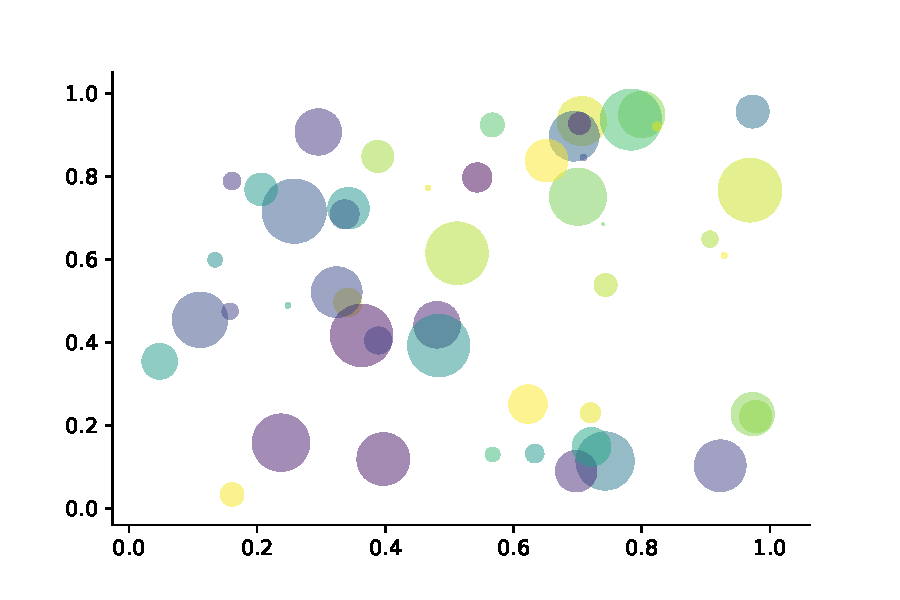
\includegraphics[width=0.6\textwidth]{scatter.pdf}
	\caption{Matplotlib: Scatter Plot Example\label{fig:mpg}}
\end{figure}

Regression analysis is a powerful statistical method that allows you to examine the relationship between two or more variables of interest. While there are many types of regression analysis, at their core they all examine the influence of one or more independent variables on a dependent variable. The process of performing a regression allows you to confidently determine which factors matter most, which factors can be ignored, and how these factors influence each other.

Let's continue using our application training example. In this case, we'd want to measure the historical levels of satisfaction with the events from the past three years or so, as well as any information possible in regards to the independent variables. 

\begin{table}[htbp]
  \small
  \centering
  \caption{Auto MPG and Price \label{tab:reg}}
    \begin{tabular}{lcc}
    \toprule
                    &       (1)         &        (2)      \\
    \midrule
    mpg             &    -238.90***     &      -49.51     \\
                    &     (53.08)       &      (86.16)    \\
    weight          &                   &      1.75***    \\
                    &                   &      (0.641)    \\
    constant        &     11,253***     &       1,946     \\
                    &     (1,171)       &      (3,597)   \\
    obs             &        74         &         74     \\
    $R^2$           &      0.220        &       0.293    \\
    \bottomrule
    \multicolumn{3}{l}{\scriptsize Standard errors in parentheses} \\
    \multicolumn{3}{l}{\scriptsize *** p<0.01, ** p<0.05, * p<0.1} \\
    \end{tabular}%
\end{table}%


\begin{itemize}[noitemsep]
  \item Routing and resource discovery;
    \begin{itemize} 
      \item Language Models
      \item Vector Space Models
    \end{itemize}
  \item Resilient and scalable computer networks;
  \item Distributed storage and search.
\end{itemize}


\section{Recruit Support Members}

Recruit support members for Elegant\LaTeX{} to translate template official guide, maintain wiki entries, update Wechat articles. No deadline for this recruitment.

So far, Elegant\LaTeX{} has four support members:
\begin{itemize}
	\item OG Translator: \href{https://github.com/peggy2006xzyz}{YPY};
	\item Wiki Maintainer: \href{https://github.com/izinngo}{Ingo Zinngo}, \href{https://github.com/xiaohao890809}{Xiaohao890809};
	\item QQ Group Manager: \href{https://github.com/sikouhjw}{Sikouhjw}.
\end{itemize}

Thank them all!!!

\section{Acknowledgement}
The number of stars on GitHub for ElegantPaper reached 176 on April 12, 2020 at the release of ElegantNote v2.20.
Thank China\TeX{} and \href{http://www.latexstudio.net/}{\LaTeX{} studio} for their promotion. 

If you like our templates, star on GitHub.
\begin{figure}[!ht]
	\centering
	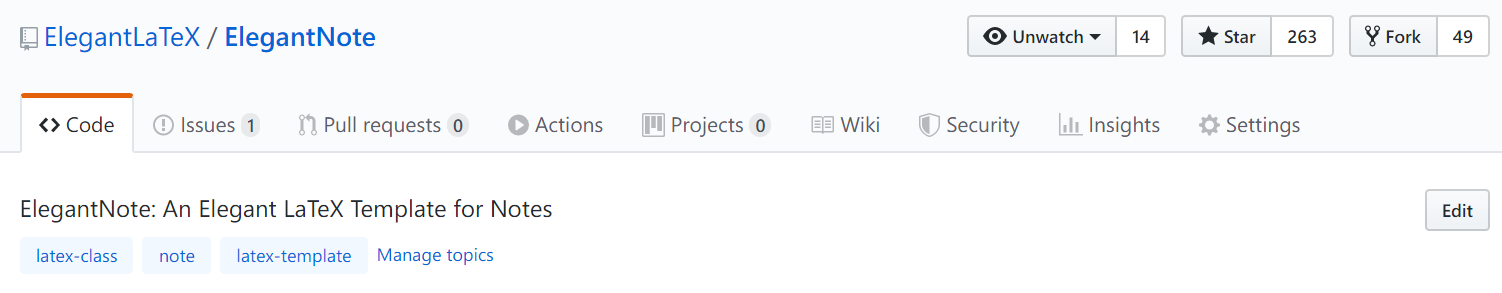
\includegraphics[width=\textwidth]{star.png}
	\caption{Twinkle, Twinkle, Little Star}
\end{figure}

\section{Donation}
To express your love for our templates and/or our developers, please do not hesitate to tip us.
\begin{figure}[!htbp]
	\centering
	
\includegraphics[width=0.4\textwidth]{donate.jpg}
\end{figure}

\textbf{The explanation right of the tip usage belongs to Elegant\LaTeX{} with no supervision. Feel free to tip us.} Those who donate more than 10 RMB will be recorded in the donation list and will receive a donation certificate. Thank all the tippers!

\begin{table}[htbp]
  \centering
  \scriptsize
  \caption{Donation List}
    \begin{tabular}{cccccccc}
    \toprule
    \textbf{Tipper} & \textbf{Amount} & \textbf{Date} & \textbf{Channel} & \textbf{Tipper} & \textbf{Amount} & \textbf{Date} & \textbf{Channel} \\
    \midrule
    Lerh  & 10 RMB & 2019/05/15 & Wechat    & yueguodipingxian & 10 RMB & 2019/05/15 & Wechat \\
	  yinsang    & 20 RMB & 2019/05/27 & Wechat    & *kong    & 10 RMB & 2019/05/30 & Wechat \\
	  latexstudio.net & 666 RMB & 2019/06/05 & Alipay   & A*n   & 40 RMB & 2019/06/15 & Wechat \\
	  * xia   & 22 RMB & 2019/06/15 & Wechat    & * qian  & 21 RMB  & 2019/06/15 & Wechat \\
	  Cassis & 11 RMB & 2019/06/30 & Wechat    & * jun    & 10 RMB & 2019/07/23 & Wechat \\
	  P*u   & 50 RMB & 2019/07/30 & Wechat    & * meng    & 19 RMB & 2019/08/28 & Wechat \\
	  Qu Doudou   & 10 RMB & 2019/08/28 & Wechat    & Li Bo    & 100 RMB & 2019/10/06 & Wechat \\
	  Njustsll & 10 RMB & 2019/10/11 & Wechat    & Liu Zhikuo   & 99.99 RMB & 2019/10/15 & Alipay \\
	  * tao   & 16 RMB & 2019/10/17 & Wechat    & Chini    & 12 RMB & 2019/10/17 & Alipay \\
	  yuanfengjing & 10 RMB & 2019/10/28 & Wechat    & Guo Deliang   & 88 RMB & 2019/11/03 & Wechat \\
	  ziqiangbuxi  & 20 RMB & 2019/11/04 & Alipay   & dushuzhichong  & 20 RMB & 2019/11/18 & Wechat \\
	  * deng    & 10 RMB & 2019/11/18 & Wechat    & * zhe   & 20 RMB & 2019/11/18 & Wechat \\
	  anonymous    & 10 RMB & 2019/11/24 & Wechat    & Jiye Qian & 66 RMB & 2019/12/04 & Wechat \\
	  * yang   & 20 RMB & 2019/12/05 & Wechat    & Catcher & 11 RMB & 2019/12/08 & Alipay \\
	  xierbotementu & 10 RMB & 2019/12/09 & Alipay   & * wei   & 10 RMB & 2019/12/09 & Wechat \\
	  Simon & 20 RMB & 2019/12/11 & Alipay   & liushangqianyi & 66.60 RMB & 2019/12/18 & Alipay \\
	  yu     & 10 RMB & 2019/12/20 & Alipay   & *chen   & 15 RMB & 2019/12/20 & Wechat \\
	  suifeng   & 20 RMB & 2019/12/27 & Alipay   & Ws    & 23.30 RMB & 2019/12/28 & Wechat \\
	  chuba    & 100 RMB  & 2020/01/02 & Alipay   & p*e   & 20 RMB & 2020/01/03 & Wechat \\
	  Shunmx & 100 RMB & 2020/01/03 & Wechat    & hj    & 10 RMB & 2020/01/03 & Wechat \\
	  F*5   & 10 RMB & 2020/01/03 & Wechat    & S*m   & 20.20 RMB & 2020/01/03 & Wechat \\
	  erdaiqingzhi  & 13 RMB & 2020/01/14 & Alipay   & *?    & 66 RMB & 2020/01/15 & Wechat \\
	  Mr. Xiong & 20 RMB & 2020/01/17 & Wechat    & *bo    & 15 RMB & 2020/01/18 & Wechat \\
	  *Zhe    & 10 RMB & 2020/02/02 & Wechat    &  Jackie &  88.80 RMB  &  2020/02/09 & Wechat \\
	  Henry\_Sun & 50 RMB & 2020/02/14 & Alipay & * Qiao  & 50 RMB & 2020/02/21 & Wechat \\
	  YunLian & 10 RMB & 2020/03/02 & Alipay & S*y  &  10 RMB  &  2020/03/15 & Wechat \\
	  * Ge  & 66.66 RMB & 2020/03/17 & Wechat    &   K*e & 30 RMB & 2020/03/30 & Wechat\\
	  * Yang  &  20 RMB  &  2020/04/02 & Wechat & Shi*n  & 30 RMB & 2020/04/11 & Wechat \\
\bottomrule
\end{tabular}%
  \label{tab:donation}%
\end{table}%


\section{FAQ}

\begin{enumerate}[label=\arabic*).]
	\item \textit{How to remove the information of version?}\\
    Please comment \lstinline|\version{x.xx}|.
	\item \textit{How to remove the information of date?}\\
	  Please type in \lstinline|\date{}|.
	\item \textit{How to add several authors?}\\
	  Use \lstinline{\and} in \lstinline{\author} and use \lstinline{\\} to start a new line.
    \begin{lstlisting}
      \author{author 1\\ org. 1 \and author 2 \\ org. 2 }
    \end{lstlisting}
\end{enumerate}


\end{document}
